\subsection{Structure du premier étage}
\label{subsec:premier_etage}

\subsubsection{Flèche}
\label{subsubsec:premier_etage}
À la suite de la conception, nous avons pu réaliser les tubes de la structure porteuse de la fusée. Nous avons procédé à un test
de flèche sur les tubes afin de nous assurer de la bonne tenue mécanique de ces derniers. Pour le tube du premier étage, nous
avons encastré le tube comme si tenu par le propulseur et réalisé les tests comme au \gls{C'Space}. 
\begin{table}[h!]
\centering
\begin{tabular}{|c|c|c|}
\hline
Positionnement & Flèche statique & Flèche dynamique \\ \hline
Patins à 0° & 0mm & 1mm \\ \hline
Patins à 90° & 0mm & 1,5mm \\ \hline
Patins à 180° & 0mm & 1mm \\ \hline
Patins à 270° & 0mm & 2mm \\ \hline
\end{tabular}
\caption{Résultats des tests de flèche du tube du premier étage}
\end{table}

Les résultats montrent une flèche maximale de 0 mm en statique et 2 mm en dynamique pour une longueur de 1 m de tube. Cela 
correspond à une flèche relative de 0 \% en statique et 0,2 \% en dynamique, ce qui est largement en dessous de la limite de
1 \% imposée par le \gls{CDC} \cite[p.~32]{CDC_BiEtage}

\subsubsection{Fabrication et collage du bloc propulsion avec ailerons}
Le bloc propulsion de SP-02 reprend la même architecture générale que celle définie pour SP-01, à savoir quatre ailerons en
fibre de verre fixés sur un tube porte-moteur intégré dans le fuselage. Le rétreint arrière est de nouveau utilisé pour
optimiser la réduction de traînée, mais le système de maintien du propulseur évolue : la vis latérale utilisée sur SP-01 est
remplacée par une bague filetée venant se visser à l’arrière du tube porte-moteur, assurant un appui axial direct sur le
propulseur. Cette modification permet de conserver la même géométrie extérieure tout en simplifiant la transmission des efforts
axiaux et en maintenant la compatibilité avec le format moteur retenu.\\

\begin{figure}[h!]
    \centering
    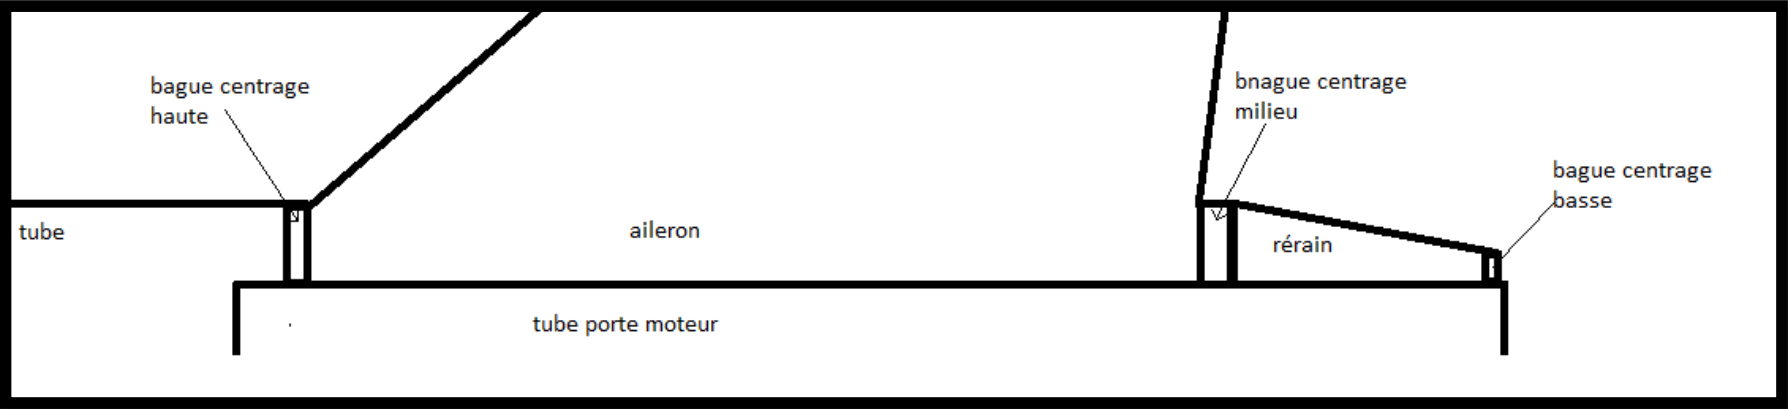
\includegraphics[width=\textwidth]{figures/schema1_SP-01.PNG}
    \caption{Procédé de collage ailerons/tube porte-moteur}
    \label{fig:collage_aileronsSP01}
\end{figure}

Le tube porte-moteur de SP-02, déjà fabriqué, reprend exactement le même principe de géométrie et de construction que celui
utilisé pour SP-01. Réalisé à partir d’un moulage sur casing Pro-54, il possède un diamètre identique au standard attendu et
conserve une longueur réduite par rapport au casing d’origine afin d’optimiser la masse tout en maintenant une rigidité
suffisante pour supporter l’ensemble du bloc propulsion. Les ailerons seront ensuite collés à la résine époxy sur ce tube déjà
réalisé, ainsi que sur les deux bagues de centrage, de manière à reproduire fidèlement la configuration mécanique utilisée
précédemment et à assurer une continuité dans l’intégration structurelle du bloc propulsion.\\

\newpage

\begin{figure}[h!]
    \centering
    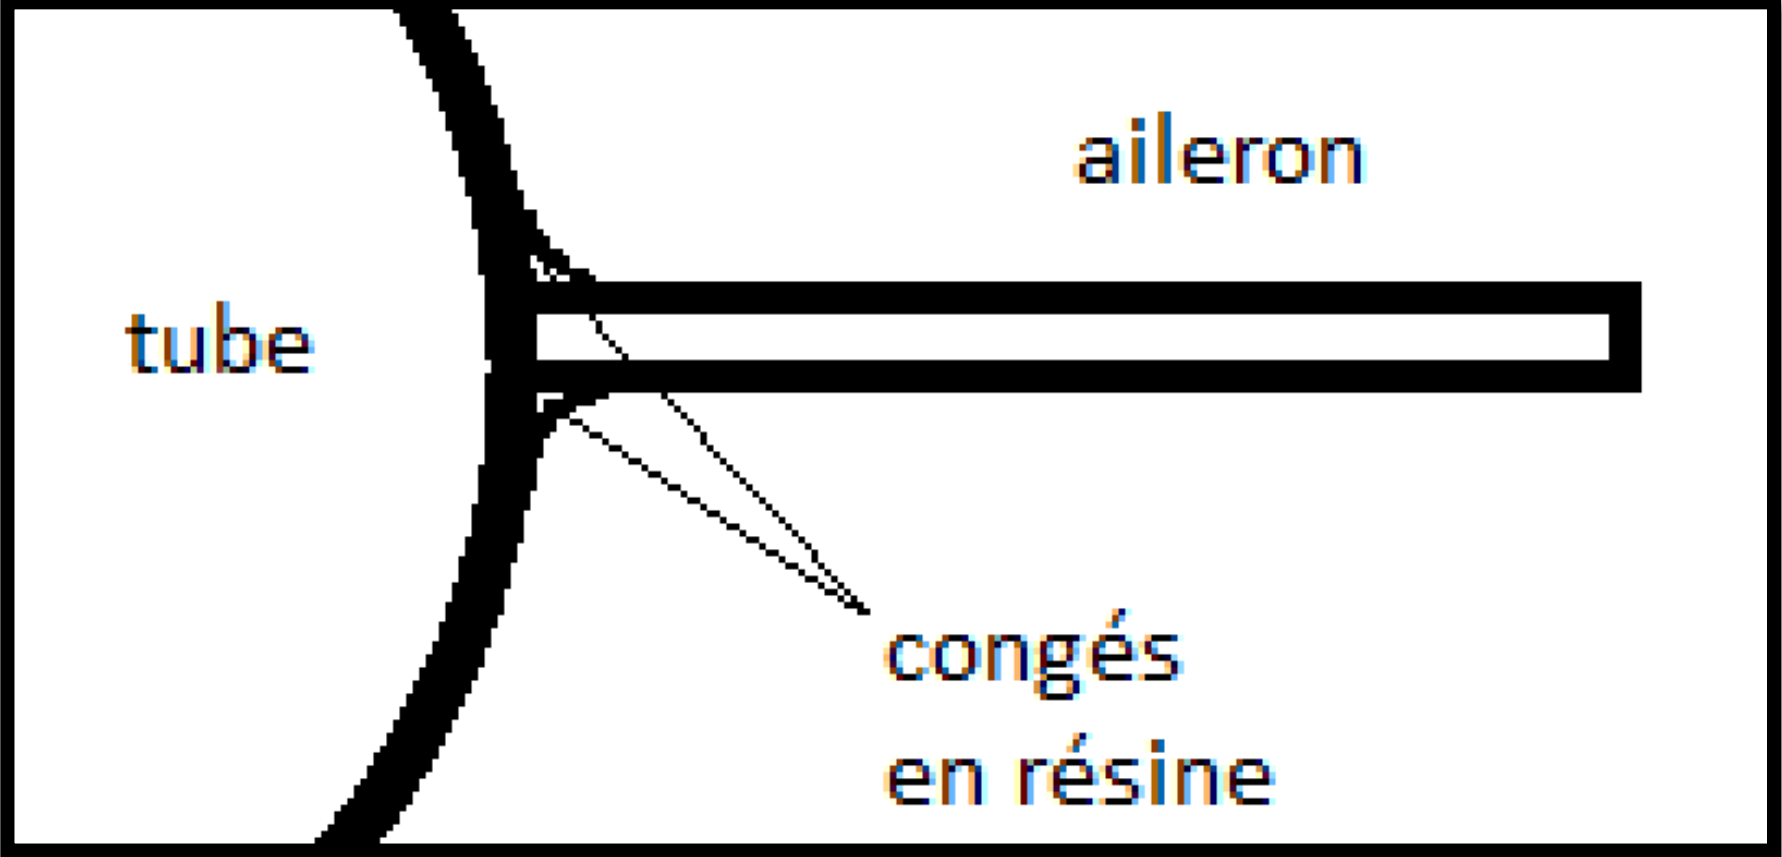
\includegraphics[width=0.5\textwidth]{figures/schema3_SP-01.PNG}
    \caption{Procédé de collage ailerons/structure avec congés en résine}
    \label{fig:collage2_aileronsSP01}
\end{figure}

Enfin, SP-02 reprend également la logique de finition appliquée sur SP-01 : des perçages seront réalisés en amont et en aval
des ailerons afin de garantir une diffusion homogène de la résine dans la zone d’assemblage, et des congés en résine seront
appliqués sur les jonctions extérieures pour assurer une transition aérodynamique lisse. Cette étape permet également de fermer
proprement les points d’injection tout en assurant une finition aérodynamique cohérente avec le modèle précédent.\\

\subsubsection{Aérofreins}
La place disponible dans le premier étage étant très limitée, nous avons opté pour un système d'aérofreins de type "plaque
déployable". Ce système est composé de deux bagues en aluminium 7075 de 7 mm d'épaisseur et du même diamètre que l'intérieur du
fuselage. Entre les deux plaques, un système de bielles permet de déployer les aérofreins à l'aide d'un servo-moteur.\\

\begin{minipage}{0.5\textwidth}
    \centering
    
\includegraphics[width=\textwidth]{figures/Catia_AF_1.png}
    \captionof{figure}{Système d'aérofrein d'SP-02 sur \acrshort{CATIA}}
    \label{fig:aerofrein_SP02}
\end{minipage}
\hfill
\begin{minipage}{0.4\textwidth}
    Une vue du système d'aérofrein d'SP-02 est présentée à la figure \ref{fig:aerofrein_SP02}. Chaque bague est vissée au corps
    de la fusée par 4 vis M4, soit 8 vis M4 pour le système complet tout, réparties uniformément. Les deux bagues sont vissées
    entre elles par 3 vis M5. Cela permet de maximisé la rigidité du système et de transmettre les efforts aérodynamiques à la
    structure principale de la fusée. Les aérofreins à proprement parler sont constitués de plaques en \gls{POMc} de 7 mm
    d'épaisseur fixés entre les deux bagues à l'intéreur de rainures usinées dans chaque bague.
\end{minipage}

\begin{minipage}{0.34\textwidth}
    La figure \ref{fig:aerofrein_SP02_ouvert_ferme} montre les deux positions possibles des aérofreins. Le déploiement se fait à
    l'aide d'un servo-moteur placé à l'intérieur du fuselage et relié aux plaques par des bièles. Une rotation de 120° des plaques
    permet de passer de la position fermée à la position ouverte.
\end{minipage}
\hfill
\begin{minipage}{0.65\textwidth}
    \begin{figure}[H]
        \centering
        \begin{subfigure}{.49\textwidth}
            \centering
            
\includegraphics[width=0.75\textwidth]{figures/Catia_AF_2.png}
            \caption{fermé}
        \end{subfigure}
        \begin{subfigure}{.49\textwidth}
            \centering
            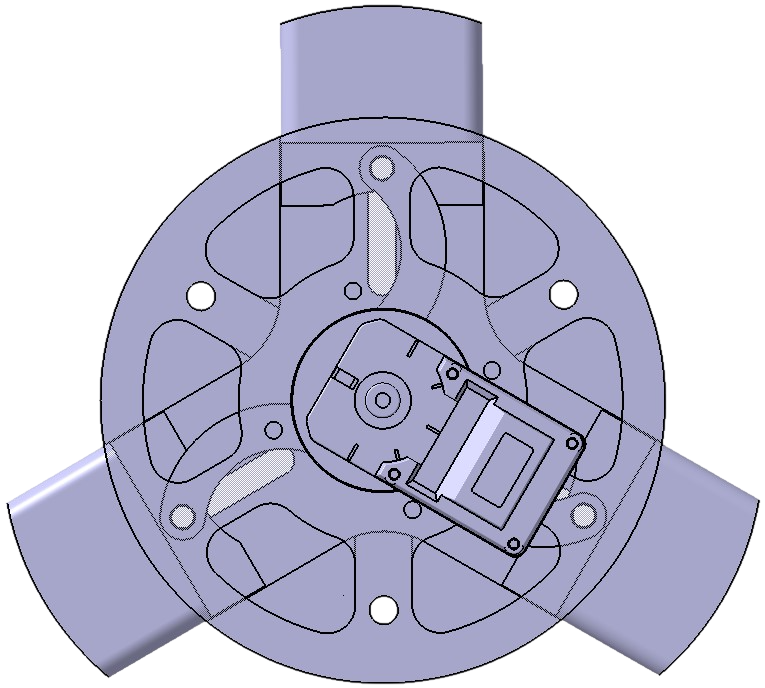
\includegraphics[width=\textwidth]{figures/Catia_AF_3.png}
            \caption{ouvert}
        \end{subfigure}
        \caption{Position des aérofreins d'SP-02}
        \label{fig:aerofrein_SP02_ouvert_ferme}
    \end{figure}
\end{minipage}

\newpage

\begin{minipage}{0.55\textwidth}
    \centering
    \begin{tikzpicture}
        
        \node at (0, 0) {
\includegraphics[width=0.8\textwidth]{figures/Catia_AF_4.png}};

        % \draw[help lines, step=1cm] (-3.5,-6) grid (6, 6);
        % \draw[help lines, step=0.5cm, lightgray] (-3.5,-6) grid (6, 6);
        % \draw[line width=2] (-3.5, +0.0) -- (+6.0, +0.0);
        % \draw[line width=2] (+0.0, -6.0) -- (+0.0, +6.0);

        \node (moteur_lbl)      at (+4.50, +4.50) {\textbf{Servo-moteur}};
        \node (rondelle1_lbl)   at (+4.50, +2.75) {\textbf{Rondelle 1}};
        \node (bague_haut_lbl)  at (+4.50, +1.75) {\textbf{Bague supérieure}};
        \node (rondelle2_lbl)   at (+4.50, +0.00) {\textbf{Rondelle 2}};
        \node (bielle_lbl)      at (+4.50, -1.00) {\textbf{Bielles (x3)}};
        \node (aerofrein_lbl)   at (+4.50, -2.00) {\textbf{Aérofreins (x3)}};
        \node (bague_bas_lbl)   at (+4.50, -4.00) {\textbf{Bague inférieure}};

        \draw [red, ->, line width=1.5] (moteur_lbl.west)     -- (-0.50, +4.50);
        \draw [red, ->, line width=1.5] (rondelle1_lbl.west)  -- (-0.25, +2.75);
        \draw [red, ->, line width=1.5] (bague_haut_lbl.west) -- (+1.50, +1.75);
        \draw [red, ->, line width=1.5] (rondelle2_lbl.west)  -- (+0.00, -1.50) -- (-0.25, -2.25);
        \draw [red, ->, line width=1.5] (bielle_lbl.west)     -- (+1.50, -2.00);
        \draw [red, ->, line width=1.5] (aerofrein_lbl.west)  -- (+2.50, -2.50);
        \draw [red, ->, line width=1.5] (bague_bas_lbl.west)  -- (+2.00, -4.00);

    \end{tikzpicture}
    \captionof{figure}{Vu éclatée du système d'aérofrein d'SP-02}
    \label{fig:aerofrein_SP02_eclate}
\end{minipage}
\hfill
\begin{minipage}{0.35\textwidth}
    La figure \ref{fig:aerofrein_SP02_eclate} présente une vue éclatée du système d'aérofrein. On y distingue les deux bagues
    en aluminium, les aérofreins en \gls{POMc}, les bielles de liaison en aluminium, les rondelles de maintien en \gls{POMc} et
    le servo-moteur. Le choix du matériau pour les aérofreins et les rondelles s'est porté sur le \gls{POMc} en raison de sa
    forte résistance mécanique, de sa facilité d'usinage et de son faible coefficient de frottement avec l'aluminium, ce qui
    réduit l'effort nécessaire pour le déploiement des aérofreins.\\
    
    La plus grande partie des pièces seront usinées au \gls{Skylab}. Seuls les aérofrein seront commandés à un fournisseur
    externe au vu de la complexité de leur forme nécessitant une fraiseuse 5 axes.
\end{minipage}

\newpage